\chapter{CƠ SỞ LÝ THUYẾT}

\section{Bộ dữ liệu và benchmark}

Nhóm tác giả \cite{ref1} chia các bộ dữ liệu thành \emph{Original Datasets} và \emph{Post-annotated Datasets}, gắn với bảy đặc tính: \emph{Cross-domain, Knowledge-augmented, Context-dependent, Robustness, Cross-lingual, Long-context} và \emph{Specialized-domain} (Bảng 2.1, trích Bảng I và Mục III-A \cite{ref1}).

\begingroup
\footnotesize
\setlength{\TableWidth}{\dimexpr\textwidth-18pt\relax}
\begin{longtable}{@{}>{\raggedright\arraybackslash}p{0.1600\TableWidth}@{\hspace{6pt}}>{\raggedright\arraybackslash}p{0.0700\TableWidth}@{\hspace{6pt}}>{\raggedright\arraybackslash}p{0.4600\TableWidth}@{\hspace{6pt}}>{\raggedright\arraybackslash}p{0.3100\TableWidth}@{}}
\caption{Đặc trưng các bộ dữ liệu chuẩn trong Text-to-SQL \cite{ref1}}\label{tab:report-1}\\
\toprule
\textbf{Bộ dữ liệu} & \textbf{Năm} & \textbf{Quy mô \& thiết lập (Bảng I, Mục III-A \cite{ref1})} & \textbf{Đặc tính (Bảng I \cite{ref1})} \\
\midrule
\endfirsthead
\toprule
\textbf{Bộ dữ liệu} & \textbf{Năm} & \textbf{Quy mô \& thiết lập (Bảng I, Mục III-A \cite{ref1})} & \textbf{Đặc tính (Bảng I \cite{ref1})} \\
\midrule
\endhead
\midrule
\endfoot
\bottomrule
\endlastfoot
\textbf{WikiSQL} & 2017 & 80.654 câu hỏi, 26.521 CSDL (1 bảng/CSDL). & Cross-domain \\
\textbf{Spider \cite{ref7}} & 2018 & 10.181 câu hỏi, 200 CSDL (5,1 bảng, 2K dòng/CSDL). & Cross-domain \\
\textbf{CoSQL} & 2019 & 15.598 câu hỏi, 200 CSDL; truy vấn qua hội thoại. & Cross-domain, Context-dependent \\
\textbf{Spider-Vietnamese} & 2020 & Bản tiếng Việt của Spider. & Cross-lingual \\
\textbf{Spider-SYN / -DK} & 2021 & Spider thay từ đồng nghĩa (SYN) / thêm tri thức miền (DK). & Robustness; Knowledge-augmented \\
\textbf{BIRD \cite{ref3}} & 2023 & 12.751 câu hỏi, 95 CSDL (7,3 bảng, 549K dòng/CSDL). & Cross-domain, Knowledge-augmented \\
\textbf{Spider 2.0 \cite{ref8}} & 2024 & 632 bài toán, 213 CSDL; LLM tiên tiến chỉ giải được 17,1\%. & Knowledge-augmented, Long-context \\
\textbf{BIRD-CRITIC} & 2025 & 600 tác vụ xử lý vấn đề thực tế trên nhiều SQL dialect. & Knowledge-augmented, Long-context \\
\end{longtable}
\endgroup

\section{Hệ thống độ đo đánh giá}

Nhóm tác giả \cite{ref1} nêu bốn độ đo thuộc hai loại, trong đó phần lớn nghiên cứu gần đây dùng độ đo \emph{execution-based} trên BIRD và các bộ họ Spider (Mục III-B). (1) \textbf{Content Matching-based}: \textbf{Component Matching (CM)} so khớp từng thành phần SQL (SELECT, WHERE, GROUP BY, ORDER BY, KEYWORDS) bằng F1-score, không xét thứ tự; \textbf{Exact Matching (EM)} là tỷ lệ câu mà mọi thành phần như ở CM đều khớp với truy vấn chuẩn. (2) \textbf{Execution-based}: \textbf{Execution Accuracy (EX)} so kết quả thực thi \emph{\ensuremath{\hat{V}_n}} của truy vấn dự đoán \emph{\ensuremath{\hat{Y}_n}} với kết quả \emph{\ensuremath{V_n}} của truy vấn \emph{ground truth} \emph{\ensuremath{Y_n}}. EX, EM chỉ được định nghĩa bằng lời; nhóm viết lại thành công thức trên \emph{N} mẫu (\ensuremath{\mathbf{1}} là hàm chỉ thị):

\begin{equation}
\mathrm{EX}=\frac{1}{N}\sum_{n=1}^{N}\mathbf{1}(V_n=\hat{V}_n),\qquad \mathrm{EM}=\frac{1}{N}\sum_{n=1}^{N}\mathbf{1}(Y_n=\hat{Y}_n)
\end{equation}

\textbf{Valid Efficiency Score (VES)} của BIRD \cite{ref3} (Eq. 1-2 \cite{ref1}) chỉ tính trên truy vấn hợp lệ (kết quả khớp \emph{ground truth}), truy vấn sai được 0 dù chạy nhanh; \emph{E(·)} là thời gian thực thi, \emph{R} lấy trung bình qua 100 lần chạy \cite{ref1}:

\begin{equation}
\begin{aligned}\mathrm{VES}&=\frac{1}{N}\sum_{n=1}^{N}\mathbf{1}(V_n=\hat{V}_n)\,R(Y_n,\hat{Y}_n),\\ R(Y_n,\hat{Y}_n)&=\sqrt{\frac{E(Y_n)}{E(\hat{Y}_n)}}\end{aligned}
\end{equation}

\section{Khung phân loại các phương pháp LLM-based Text-to-SQL}

Nhóm tác giả \cite{ref1} chia các phương pháp thành hai \emph{paradigm} (Hình 2.1): \textbf{In-context Learning (ICL)} và \textbf{Fine-tuning (FT)}. Theo góc độ cài đặt, ICL gồm C0 và bốn loại C1-C4: \textbf{C0-Vanilla Prompting} (\emph{zero-shot, few-shot}); \textbf{C1-Decomposition} (\emph{multi-module collaboration, question decomposition}); \textbf{C2-Prompt Optimization} (\emph{advanced few-shot sampling, schema augmentation, external knowledge integration}); \textbf{C3-Reasoning Enhancement} (\emph{CoT-based, consistency-driven, program-based and tool-augmented reasoning}); \textbf{C4-Execution Refinement} (\emph{feedback-driven regeneration, execution-guided selection}). Các loại đều giữ nguyên \emph{\ensuremath{\theta}}, phần lớn dựa trên \emph{zero-shot prompt} \emph{\ensuremath{P_0}} hoặc \emph{few-shot prompt} \emph{\ensuremath{P_k}} với \emph{k} ví dụ \emph{\ensuremath{\mathcal{E}_i}} = (\emph{\ensuremath{S_i}}, \emph{\ensuremath{Q_i}}, \emph{\ensuremath{Y_i}}) (Eq. 4-5, \ensuremath{\oplus} là phép nối):

\begin{equation}
P_0=I\oplus S\oplus Q,\qquad P_k=\{\mathcal{E}_1,\mathcal{E}_2,\ldots,\mathcal{E}_k\}\oplus P_0
\end{equation}

\begin{figure}[htbp]
\centering
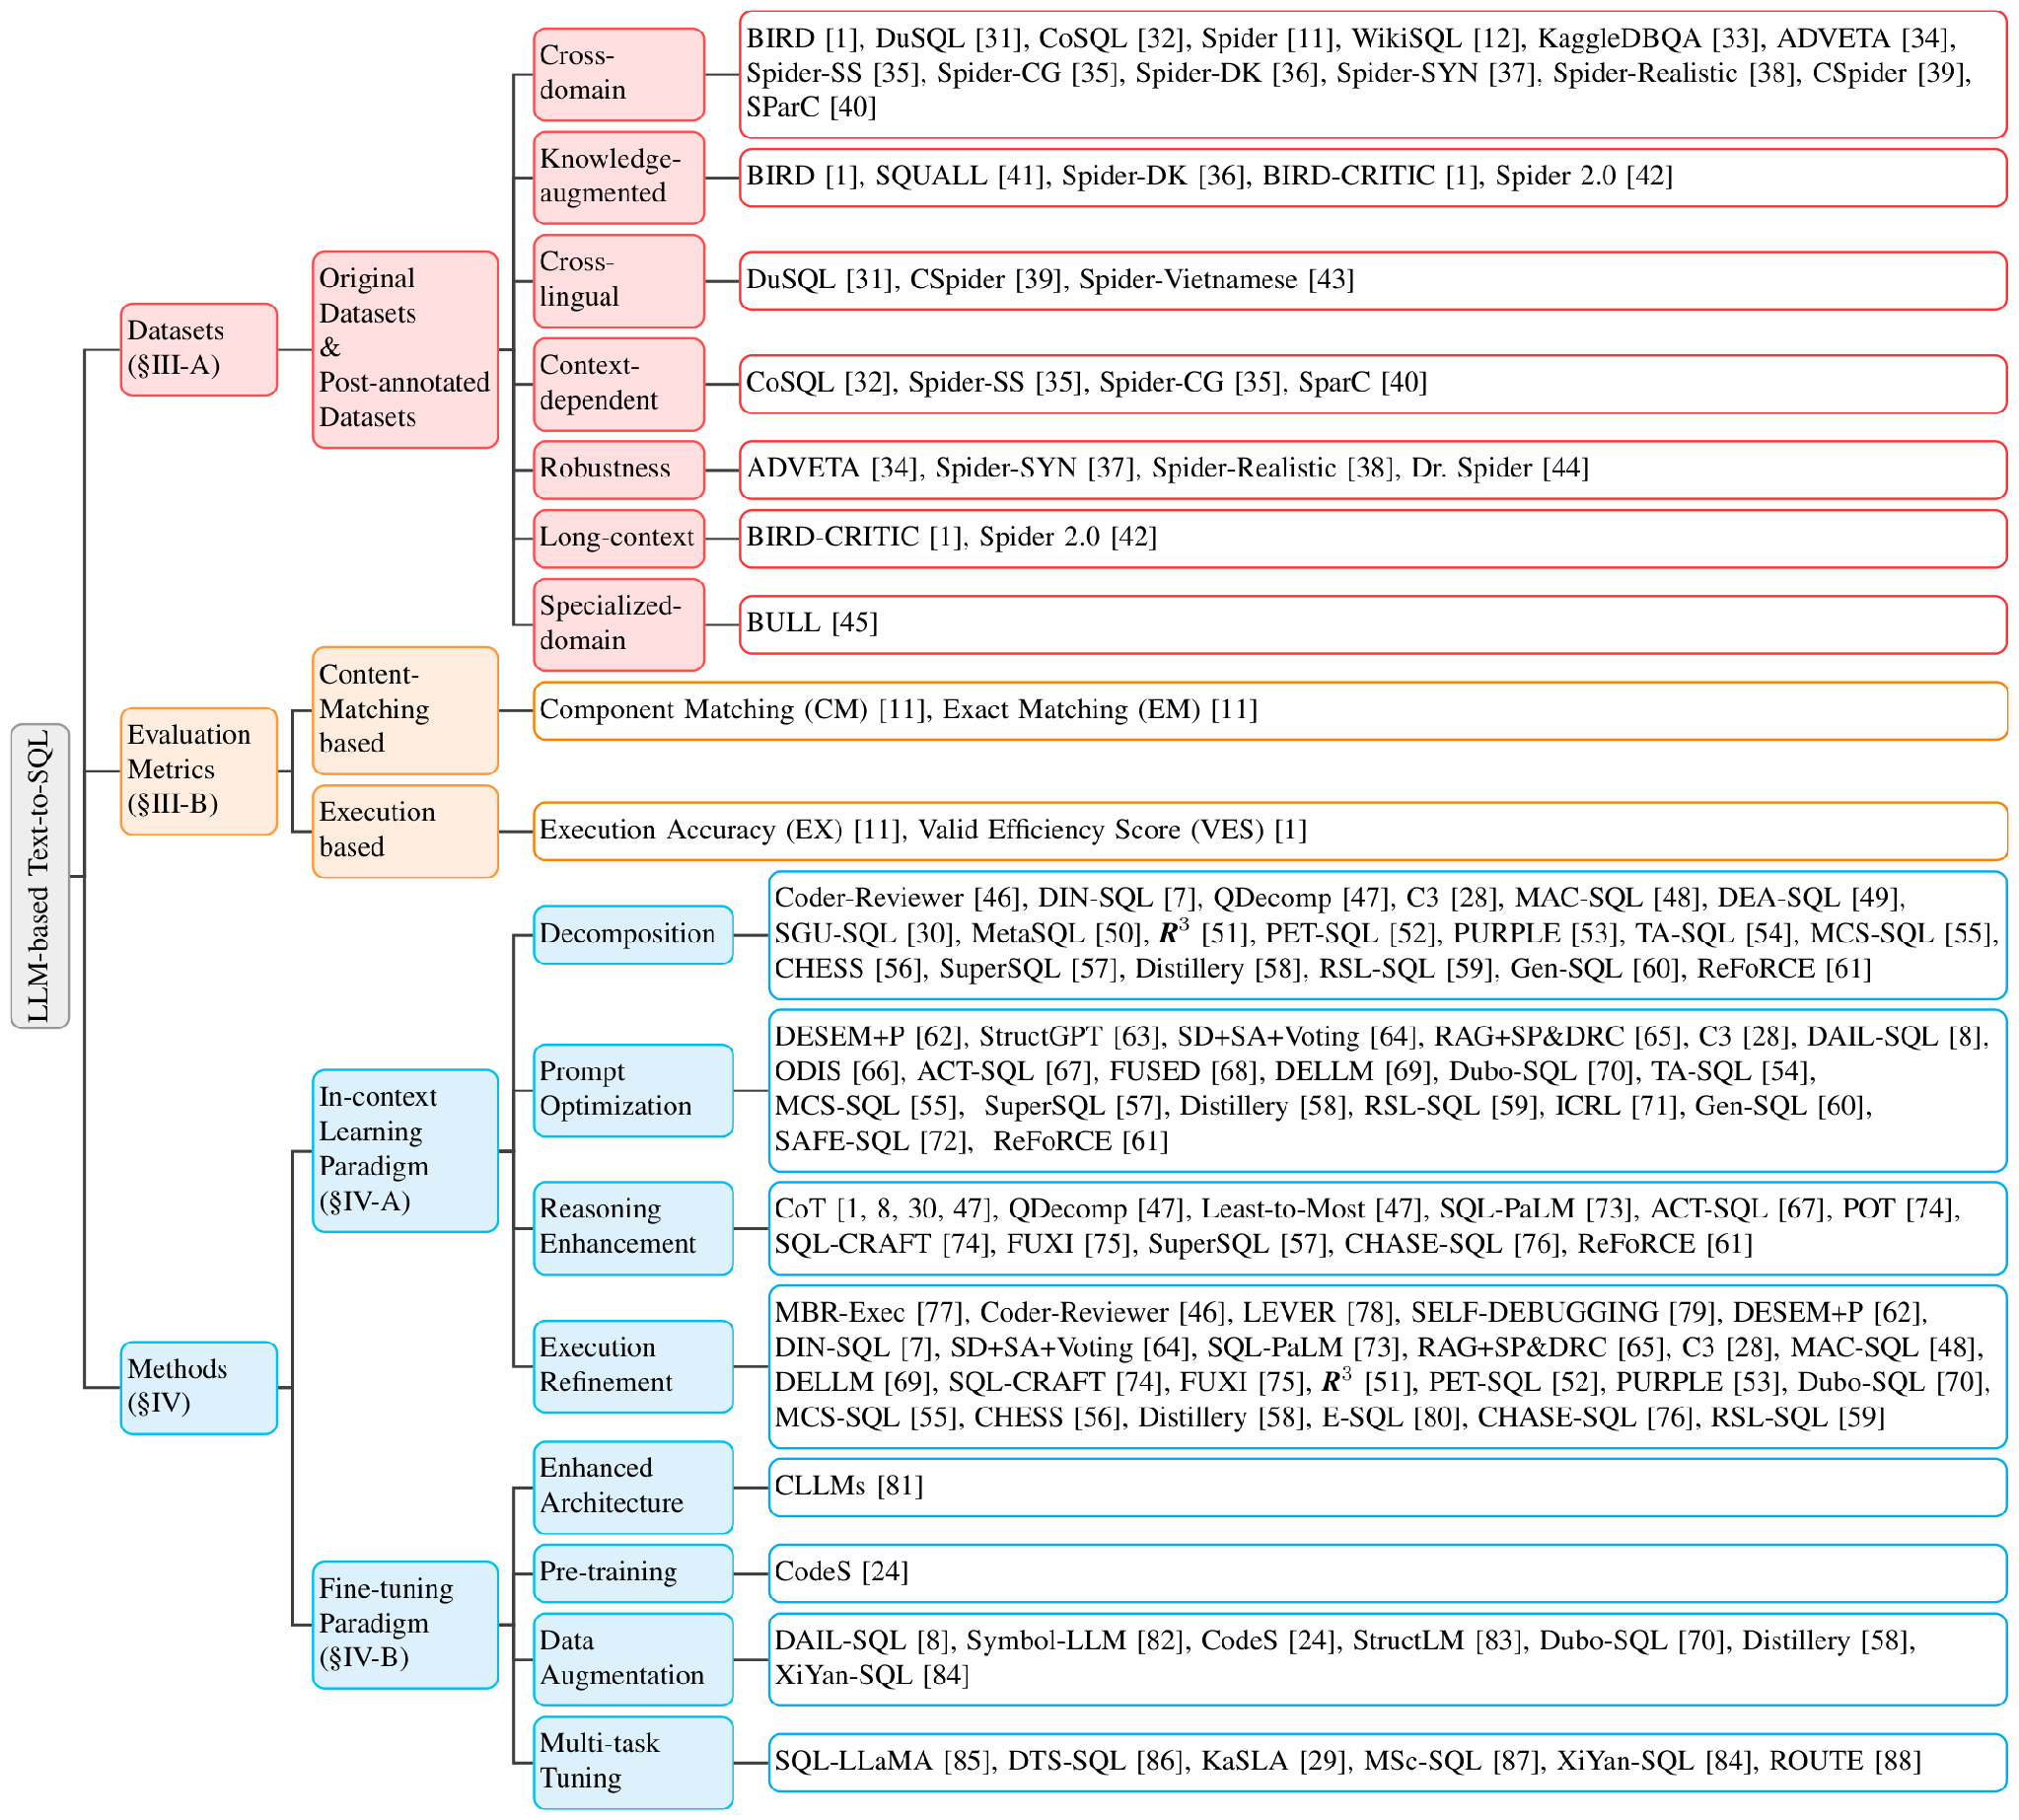
\includegraphics[width=\linewidth,height=0.68\textheight,keepaspectratio]{03-method-taxonomy}
\caption{Khung phân loại các phương pháp LLM-based Text-to-SQL \cite{ref1}}\label{fig:03-method-taxonomy}
\end{figure}

Theo cơ chế huấn luyện, \textbf{FT} gồm bốn loại \cite{ref1}: \textbf{Enhanced Architecture} (CLLMs \cite{ref9}); \textbf{Pre-training} (CodeS \cite{ref10}); \textbf{Data Augmentation} (DAIL-SQL \cite{ref5}); \textbf{Multi-task Tuning} (SQL-LLaMA của MAC-SQL \cite{ref6}). ICL vẫn chủ đạo vì LLM mã nguồn mở kém LLM thương mại khi hiểu CSDL phức tạp. FT thường cập nhật \emph{\ensuremath{\theta}} bằng \emph{supervised fine-tuning} (SFT), cực tiểu \emph{cross-entropy loss} trên \ensuremath{\mathcal{D}} (Eq. 7); \emph{P} là \emph{prompt} ở (4), \emph{Y} = [\emph{y1}, …, \emph{yT}] là SQL \emph{ground truth}:

\begin{equation}
\mathcal{L}_{\mathrm{SFT}}=-\sum_{(P,Y)\in\mathcal{D}}\sum_{t=1}^{T}\log\Pr_{\pi}\!\left(y_t\mid P,y_{<t}\right)
\end{equation}

